%vormatierung
\documentclass[12pt,a4paper,bibliography=totocnumbered,listof=totocnumbered]{scrartcl}
%zeilenabstand
\usepackage{setspace}
\onehalfspacing
\parindent 0pt

\usepackage{tabularx}
\usepackage[utf8]{inputenc}
%font änder
\usepackage[ngerman]{babel}
%ränder
\usepackage[paper=a4paper,left=40mm,right=30mm,top=25mm,bottom=25mm]{geometry} 
%Abstand Fusnoten
\deffootnote{1em}{1em}{\textsuperscript{\thefootnotemark\ }}
%sub und subbubsection tiefe
\setcounter{tocdepth}{3}
%Inhaltsverzeignis anklickbar.
\usepackage{hyperref}
\setcounter{secnumdepth}{3}
%sonderzeichen
\usepackage[T1]{fontenc}
%grafiken einbinden
\usepackage{graphicx}
\usepackage{pdflscape}
\usepackage{listings}

\lstdefinestyle{myStyle}{
    backgroundcolor=\color{gray!10},   % Hintergrundfarbe
    basicstyle=\ttfamily\small,        % Schriftart und -größe
    frame=single,                      % Rahmen um den Text
    framesep=5pt,                      % Abstand zwischen Rahmen und Text
    rulecolor=\color{black},           % Rahmenfarbe
    xleftmargin=10pt,                  % Abstand vom linken Rand
    xrightmargin=10pt,                 % Abstand vom rechten Rand
    breaklines=true,                   % Zeilenumbruch zulassen
    breakatwhitespace=true,            % Zeilenumbruch an Leerstellen
    showstringspaces=false,            % Leerzeichen in Strings nicht hervorheben
}


%Wie können künstliche Intelligenzen bei der Entwicklung eines Videospiels in der Unreal Engine 5 eingesetzt werden?
\title{Entwicklung eines Videospielprototypen als ,,Ein-Mann-Videospielentwickler´´ auf der Unreal Engine 5 mit Hilfe von KI-Systemen}

\author{Nicolas Taylor}

\date{11.04.2023}

\begin{document}
\thispagestyle{empty}
\begin{center}
	
	\vspace*{1cm}
	\Large
	\textbf{Hochschule Fulda}\\
	\textbf{Fachbereich Angewandte Informatik}\\
	\vspace*{4cm}
	
	\huge
	\textbf{BA}\\
	\vspace*{0.5cm}
	\large
	
	\textbf{Entwicklung eines Videospielprototypen als ,,Ein-Mann-Videospielentwickler´´ auf der Unreal Engine 5 mit Hilfe von KI-Systemen}\\
	\vspace*{1cm}
%	\includegraphics[scale=1.0]{Bilder/logo.png}\\
%	\vspace*{2cm}
	
	\vfill
	\normalsize
	\newcolumntype{x}[1]{>{\raggedleft\arraybackslash\hspace{0pt}}p{#1}}
	%\begin{tabular}{x{6cm}p{7.5cm}}
		%\rule{0mm}{5ex}\textbf{Autor:} & Nicolas Taylor - nicolas.taylor@gmx.net
		%rule{0mm}{5ex}\textbf{Prüfer:} & Prof. Dr. Christian Fischer
		%\\
		%\rule{0mm}{5ex}\textbf{Abgabedatum:} & 11.04.2023
		%\\
	%\end{tabular}
\end{center}
\pagebreak
\tableofcontents
\newpage
%1
\section{Einleitung}
Sprich mir nach; ich bin Game Designer. Herzlichen Glückwunsch, du bist "Gamedesigner."
\\
Dieses Zitat stammt von Jesse Schell; Hochschullehrer für Unterhaltungstechnologie am Entertainment Technology Center in Pittsburgh, USA.
\\
Wenn er gefragt wird, was er macht, um seine Brötchen zu verdienen, antwortet er: "Ich bin Game Designer". Jesse Schell, ermutigt Anfänger in seinem Buch, die noch vor Ihrem ersten Schritt Game Designer oder Videospiele Entwickler stehen, sich selbst als Gamedesigner zu bezeichnen. Wenn wir den Worten von Jesse Schell Glauben schenken, ist Gamedesigner werden nicht schwer, aber ein Videospiel zu entwickeln ist hingegen sehr.
\\
Wenn man sich dazu entscheidet Videospiele zu produzieren, steht man am Anfang sehr oft alleine da. Genau um dieses alleine zu sein, möchte ich mich auf meine Bachelor Thesis beziehen. Ich benutze in meiner Bachelorthesis den Begriff Ein-Mann-Videospielentwickler, um zu verdeutlichen, dass alle Prozesse an einer Person abhängen.
\\
In der Videospielindustrie ist es heute üblich, dass ein Spiel von Entwickler Studios entwickelt wird, die mehrere hundert Angestellte haben. Zum Beispiel Baldur´s Gate 3 , was von dem Belgischen Entwicklerstudio Larian Studios entwickelt wurde, hat mehr als 450 Angestellte.
\\
Im Jahr 2022 hat ein großes kulturelles Umdenken in unserer Gesellschaft stattgefunden, was das Thema KI angeht. Früher ein Thema für Nerds und Science Fiction, heute ein Thema für Markus Lenz und die Tagesschau.
\\
Bettina Stark-Watzinger bezeichnet KI als Schlüsseltechnologie.
\\
Mein Ziel ist es, als Ein-Mann-Videospielentwickler einen Prototyp im Rahmen meiner Bachelorthesis zu entwickeln mit Hilfe von KI-Systemen.
\\
Genau diese Entwicklung möchte ich in meiner Thesis analysieren und beschreiben.
%https://dailygame.at/baldurs-gate-3-entwickler-bleibt-weiterhin-unabhaengig/ -03.09.2023
\subsection{Motivation und Idee}
Videospiele zu entwickeln ist eine Aufgabe, die großes Know-How voraussetzt. In den größten Videospiel Studios ist es kein Einzelfall, dass über 500 Menschen angestellt sind.
\\
Videospiele werden aus sehr vielen Teilbereichen der Medienbranche zusammengesetzt, wie zum Beispiel Autoren, Programmierer und Illustratoren bis hin zu Marketing und Vertrieb.
\\
In den Anfangszeiten, wo Videospiele gerade angefangen haben, sich kommerziell als Unterhaltungsmedium zu etablieren, wurde ein großer Teil von Videospielen von einer Person geschrieben. Spiele Wie Space Invader, Adventure oder Space War [arbeitstitel bitte noch mal in der geschichte der VS nachssacuen]
\\
Spätestens in den 90er Jahren wurden nur noch sehr wenige Spiele von einer Person entwickelt. Die Systeme, auf denen Videospiele liefen, wurden immer leistungsfähiger, und somit wurden auch lebendigere und komplexere Welten möglich. Videospiele wurden in der Regel nicht mehr von einer Person entwickelt, sondern von ganzen Studios. In diesen Studios werden Aufgaben auf Teams verteilt, wie zum Beispiel Concept Art and Design, Musik und Soundeffekte bis hin zum Vertrieb und Marketing.
\\
Kurz, ein Videospiel zu entwickeln ist schon sehr lange keine Ein-Mann-Aufgabe mehr, Und in solchen Teams kann jeder Videospielentwickler sich auf seine Stärken im Team konzentrieren.
\\
Ich sehe seit 2022 eine neue Möglichkeit Videospiele zu entwickeln, die zuvor in diesem Umfang nicht möglich gewesen war.
\\
KI-Systeme sind Werkzeuge, die ein hohes Potenzial beinhalten, um schnelles und qualitatives Arbeiten mit sich bringen.
\\
Mit Midjourney kann ich innerhalb von wenigen Minuten eine Landschaft erstellen lassen. ChatGPT kann dir Geschichten schreiben und Voice.ai dir eine neue Stimme verleihen. Das was die vorhin drei genannten KI-Systeme sich spezialisiert haben, sind in der realen
Welt, echte Berufe in der Gamingbranche - Concept Artist, narrative Designer / video game writer, voice actor.
\\
Es ist heute theoretisch möglich, ohne viele Vorkenntnisse diese Aufgaben mit Hilfe von KI-Systemen zu übernehmen.
\subsection{Forschungsfrage}
\subsection{Forschungsmethoden}
Ich werde in dieser Arbeit einen Prototyp entwickeln. Während dieser Arbeit werde ich versuchen, Probleme und Aufgaben mit KI-Systemen zu lösen. Diese Lösungen werde ich in dieser Arbeit präsentieren.
\subsection{Gliederung der Arbeit}%todo hööööö?!
Die Arbeit ist gegliedert in, Warum ich was mache, dann ein Paar allgemeine Erklärungen.
\\
Was ich mache. Und welche Werkzeuge ich benutze. Ich werde Alles am Ende analysieren
\subsection{Zielsetzung}
Mein Ziel in dieser Arbeit ist es, einen Prototyp zu entwickeln. Dieser Prototyp wird nur von einer Peron entwickelt, und alle anderen Aufgaben und Probleme werden versucht, mit Hilfe von KI-Systemen zu lösen.
\subsection{Abgrenzung}
%2
\section{Theoretischer Hintergrund}
%\\\\\\\\\\\\\\\\\\\\\\\\\\\\\\\\
\subsection{Begriffsdefinitionen}%erläuterung
%\\\\\\\\\\\\\\\\\\\\\\\\\\\\\
\subsubsection{KI-System}
%https://www.bsi.bund.de/DE/Themen/Verbraucherinnen-und-Verbraucher/Informationen-und-Empfehlungen/Technologien_sicher_gestalten/Kuenstliche-Intelligenz/kuenstliche-intelligenz_node.html
Mittels maschinellen Lernens großer Datenmengen, können KI-Systeme, selbständige Lösungskompetenzen erwerben. KI-Systeme können die Fähigkeit besitzen, Eingabedaten, die nicht zu ihren Trainingsdaten vorkommen, zu verarbeiten.
\subsubsection{Prompt}
%https://dict.leo.org/englisch-deutsch/prompts ; https://bm-experts.de/definitionenfaq/definitionen/prompt-was-ist-das-und-wie-kann-er-eingesetzt-werden/
Aus dem Englischen, to prompt, und bedeutet so viel wie auordern oder ab fragen. Der User benutzt Prompts, um einem KI-System einen Befehl zu überreichen. Im Beispiel von ChatGPT gibt der User ein Prompt in das Chatfenster, undb ChatGPT generiert eine passende Antwort.
\subsubsection{NPC}
% (DKDG) Klaus Breuer - Computerspiele programmieren - Künstliche Intelligenz für Künstliche Gehirne - Kapitel 15.1 Erster Absatz Seite 113 ------ Computerspiele programmieren: künstliche Intelligenz für künstliche Gehirne / Breuer, Klaus Barcode 12155751 Rückgabe bis 12.06.2023
Non-Player Characters, kurz NPC, sind vom Computer gesteuerte Charaktere, Dorfbewohner, Tiere oder sogar Monster. Alle Charaktere und Tiere, die sich nicht vom Spieler kontrollieren lassen. NPCs sind notwendig, um eine Spielwelt lebendig wirken zu lassen.
\subsubsection{Game Designer}
%Die Kunst des Game Designs : bessere Games konzipieren und entwickeln / Schell, Jesse Barcode 12486880 Kapitel 1.2 Seite 35 bis 37 DKDG
Ein Game Designer besitzt ein breites Spektrum an Fähigkeiten wie Animation, Architektur, Betriebswirtschaft, Game Engineering, Darstellende Kunst, Geschichte, Management, Mathematik, Musik, Präsentation, Soundgestaltung, Spiele und viele weitere beherrschen sollte.
\\
Der Game Designer erschafft ein Erlebnis, wobei das Spiel nicht das Erlebnis ist, sondern nur die Möglichkeit, dem Spieler ein Erlebnis zu erleben.
%Kapitel 2.1 Seite 44
\subsubsection{Design}%Seite 49 oder eine andere gemeingültige Quelle DKDG
\subsubsection{Spiel}%Kapitel 4.2 seite 74 bis 89-- Großes Kapitel
\subsection{Videospiel-Entwicklung}
\subsubsection{Die Vier Grundelemente eines Videospiels}%Kapitel5.2 Seite 93 DKDG
\subsection{Unreal Engine 5}
%https://www.unrealengine.com/de/unreal-engine-5 abrufdatum 27.05.2023
Die Unreal Engine ermöglicht den Spieleentwickler 3D-Videospiele zu entwickeln. Die Entwicklung eines Videospiels in der Unreal Engine 5 kann in Echtzeit entwickelt werden, das bedeutet, dass man das Ergebnis seiner Arbeit sofort betrachten kann. Epic Games, die Entwickler der Unreal Engine 5, beschreiben sie als "Das weltweit offenste und fortschrittlichste Tool zur 3D-Erstellung in Echtzeit".
\subsubsection{Narnite}
\subsubsection{Lumen}
\subsection{Künstliche Intelligenz und ihre Anwendungen in der Videospiel-Entwicklung}
\subsection{Vor- und Nachteile des Einsatzes von KI in der Videospiel-Entwicklung}
%3
\section{Methodik}
\subsection{Auswahl und Beschreibung der KIs}
\subsubsection{ChatGPT}
\subsubsection{Midjourney}
\subsubsection{PIFuHD}
\subsubsection{Voice.AI}
\subsubsection{Adobe Enhanced Speech}
\subsection{Beschreibung der Tools und Technologien}
\subsubsection{Blender}
\subsubsection{Audacity}
\subsection{Beschreibung des Entwicklungsprozesses}
%4
\section{Umsetzung}
\subsection {Idee und Konzeption}
Meine Idee ist ein Videospiel zu entwickeln, das eine geschichtliche und kulturelle Relevanz zur deutschen Geschichte hat. Ein weiteres Kriterium an meinem Videospiel ist es, ein Szenario zu wählen, das sich vor dem Zweiten Weltkrieg befindet. Mit dieser Idee ging ich zu ChatGPT und habe folgenden Prompt formuliert und anschließend diese Ausgabe bekommen.
\begin{figure}[h]
	\centering
	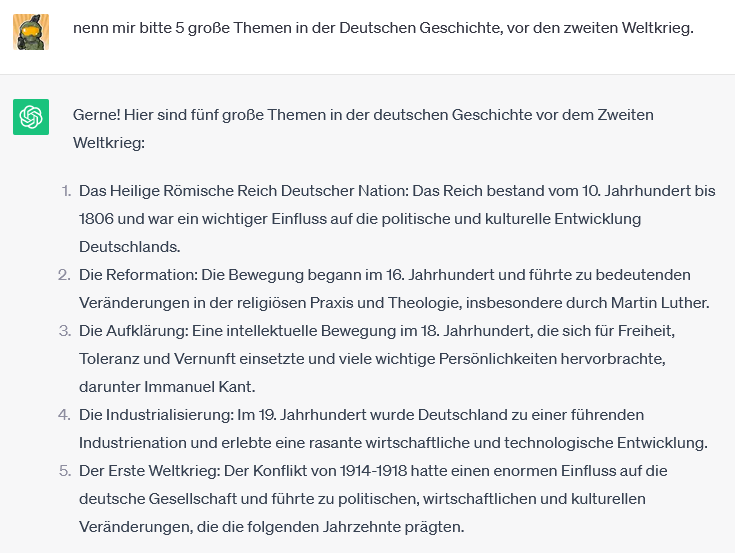
\includegraphics[scale=0.7]{BilderFuerBA/CGPTBachelorarbeitZurKI/01.png}
	\caption{Ersten 5 Themen}
	\label{fig:ersten-5-themen}
\end{figure}
\begin{figure}[h]
	\centering
	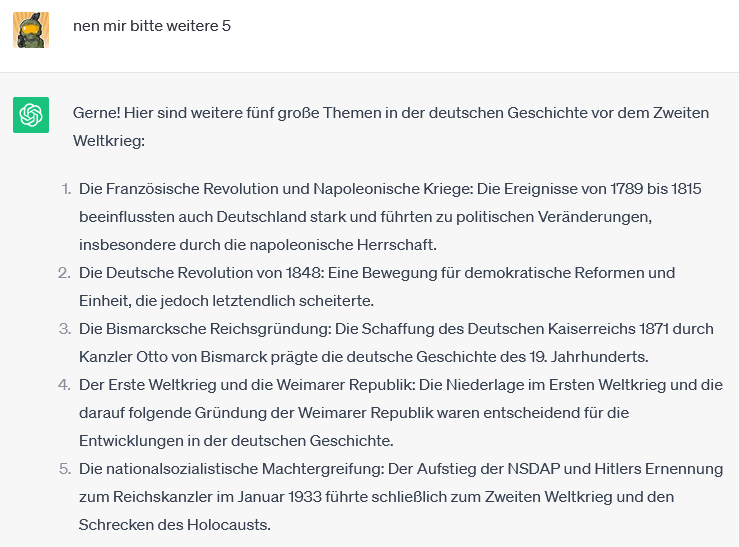
\includegraphics[scale=0.7]{BilderFuerBA/CGPTBachelorarbeitZurKI/02.png}
	\caption{Zweiten 5 Themen}
	\label{fig:zweiten-5-themen}
\end{figure}
Man kann an diesem Beispiel sehen, dass ChatGPT. ChatGPT hat mir in diesem Fall sehr schnell geholfen mir 10 Ideen präsentiert, die ich in meinem Videospiel verarbeiten kann.
Als Ein-Mann-Videospielentwickler entschied ich mich für die Reformation mit Martin Luther als Hauptfigur.
\\
Innerhalb dieser Bachelorthesis ist es mir aus Zeitgründen nicht möglich ein komplettes Videospiel zu entwickeln, was das Leben von Martin Luther widerspiegelt. Durch meine Recherche über Martin Luther und sein Leben fand ich eine Moment sehr bedeutend, und zwar den Moment, wo Martin Luther seine 96 Thesen an das Kirchtor nagelt.
\\
In meinem Prototyp werde ich dieses Ereignis als Thematischen Mittelpunkt wählen.
Meine Spielidee für meinen Prototyp ist nun, dass Martin Luther durch ein Dorf läuft, verschiedene NPCs trifft und mit ihnen in einen Dialog tritt. Martin Luther trifft verschiedene Personen mit verschiedenen Problemen und Ansichten. Er redet mit ihnen und lässt sich von ihnen inspirieren. Durch diese Inspiration entwickelte Martin Luther, später im Spiel, seine 96 Thesen.
\\
Kern des Prototyps ist die Entwicklung einer Spielwert, die aus einem Dorf mit verschiedenen Häusern und NPCs besteht.
\\
Die Entwicklung des Prototyps unterteilt sich in verschiedene Meilensteine:
-Hauptfigur
\\
-Landschaft
\\
-Gebäude
\\
-Nebenfiguren
\\
-Dialogsystem
\\
-Sprachausgabe
\\
Jeder dieser Meilensteine besitzt in dieser Theses sein eigenes Kapitel, in dem die Entwicklung nahe gebracht wird.
\subsection {Meilenstein: Hauptfigur}
\begin{figure}[h]
	\centering
	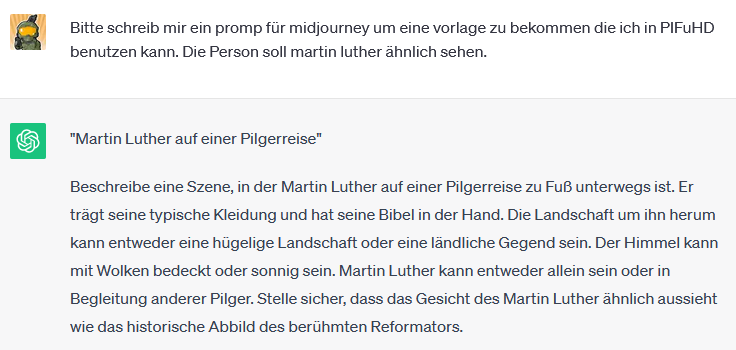
\includegraphics[scale=0.7]{BilderFuerBA/CGPTMidJourneyMartinLuther/01.png}
	\caption{Erster Versuch: ChatGPT erstellt Promt für Midjourney}
	\label{fig:chatgpt-ptompt-Midjourney-01}
\end{figure}
\begin{figure}[h]
	\centering
	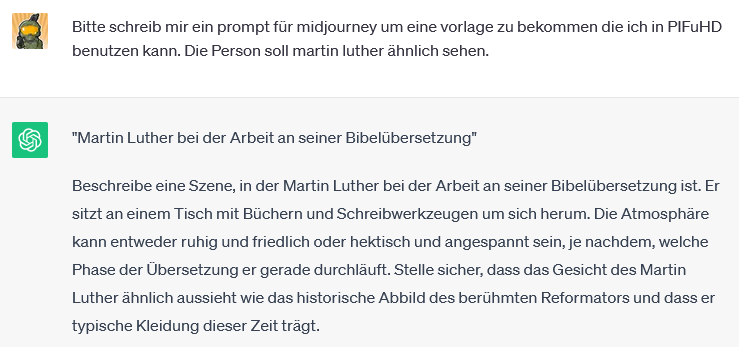
\includegraphics[scale=0.7]{BilderFuerBA/CGPTMidJourneyMartinLuther/02.png}
	\caption{Zweiter Versuch: ChatGPT erstellt Promt für Midjourney ohne Rechtschreibfehler}
	\label{fig:chatgpt-ptompt-Midjourney-02}
\end{figure}
\begin{figure}[h]
	\centering
	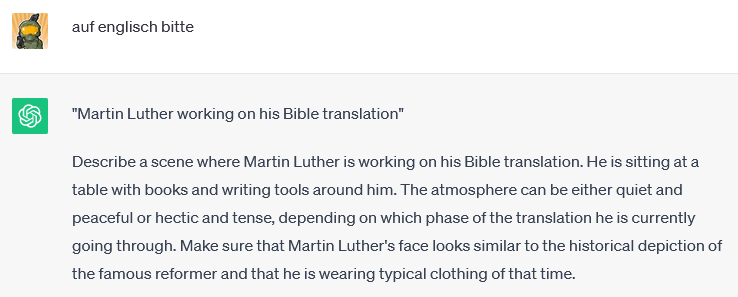
\includegraphics[scale=0.7]{BilderFuerBA/CGPTMidJourneyMartinLuther/03.png}
	\caption{Dritter Versuch: ChatGPT erstellt Promt für Midjourney in Englisch}
	\label{fig:chatgpt-ptompt-Midjourney-03}
\end{figure}
Der erste Versuch hat einen deutschen Prompt ausgegeben, der anschließend übersetzt wurde.
\\
Dieser Prompt wurde Midjourney übergeben, was diese Bilder als Resultat ergibt.
[BILD]
ChatGPT beschrieb sehr atmosphärisch, was in ein sehr unaufgeräumtes Resultat hervorbringt.
Es wird vermutet, dass ChatGPT nicht genügend darauf trainiert ist, wie Midjourney Prompts auszusehen sind.
\\
Eine Recherche auf YouTube hat gezeigt, dass das verwenden von Midjourney-Formeln ein aufgeräumtes Ergebnis hervorrufen kann. Diese Formel wurde ChatGPT übergeben und er hat sie vermutlich verstanden.
\begin{figure}[h]
	\centering
	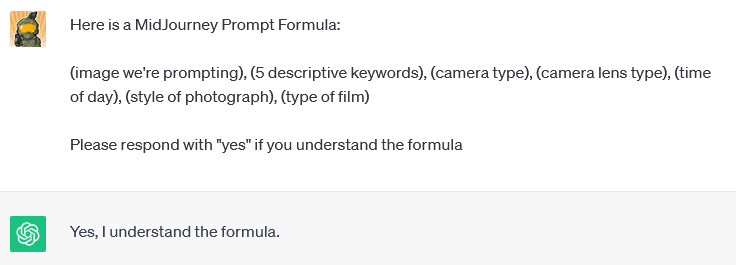
\includegraphics[scale=0.7]{BilderFuerBA/CGPTMidJourneyMartinLuther/04.png}
	\caption{Vierter Versuch: Aufforderung ChatGPT verwendung einer Midjourney-Formel}
	\label{fig:chatgpt-ptompt-Midjourney-04}
\end{figure}
\begin{figure}[h]
	\centering
	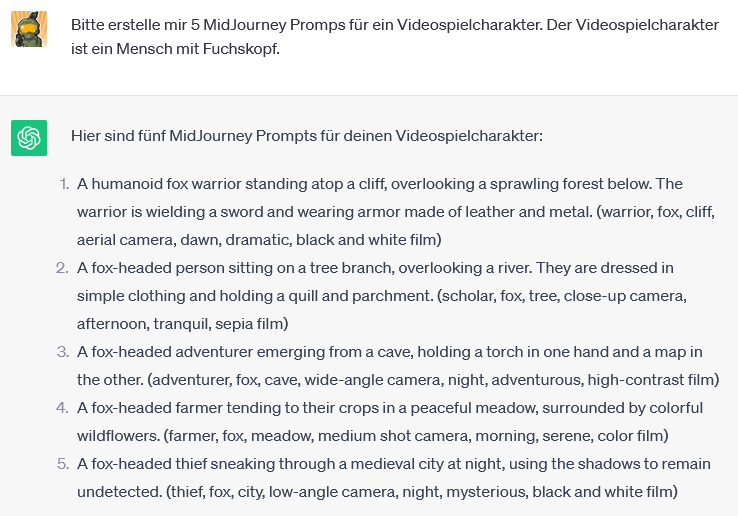
\includegraphics[scale=0.7]{BilderFuerBA/CGPTMidJourneyMartinLuther/05.png}
	\caption{Erster Test MJ-Formel: ChatGPT erstellt Promt mit verwendung der Midjourney-Formel}
	\label{fig:chatgpt-ptompt-Midjourney-05}
\end{figure}
\begin{figure}[h]
	\centering
	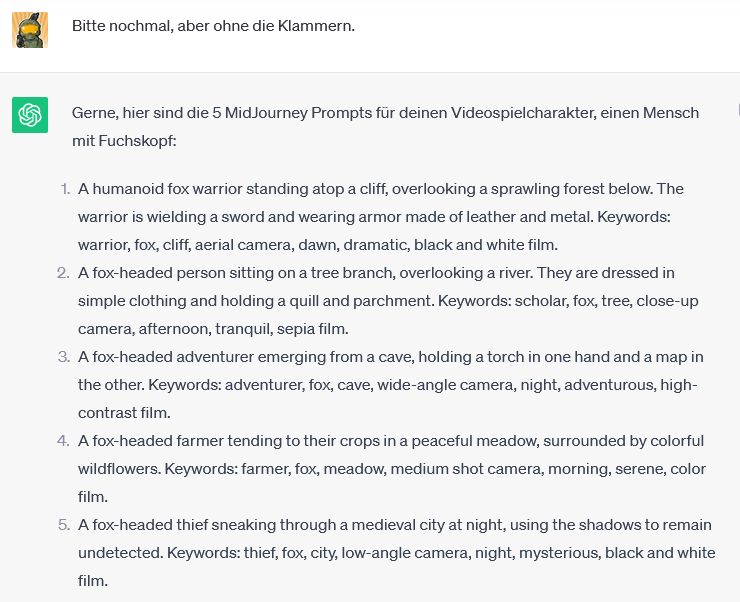
\includegraphics[scale=0.7]{BilderFuerBA/CGPTMidJourneyMartinLuther/06.png}
	\caption{Zweiter Test MJ-Formel: ChatGPT erstellt Promt für Midjourney in Englisch ohne Klammern}
	\label{fig:chatgpt-ptompt-Midjourney-06}
\end{figure}
Im ersten Test werden die Prompts mit Klammern ausgegeben. Diese sind mit einer einfachen Aufforderung möglich zu entfernen
%[BILD]
%[BILD]
\subsection {Meilenstein: Gebäude}
\begin{figure}[h]
	\centering
	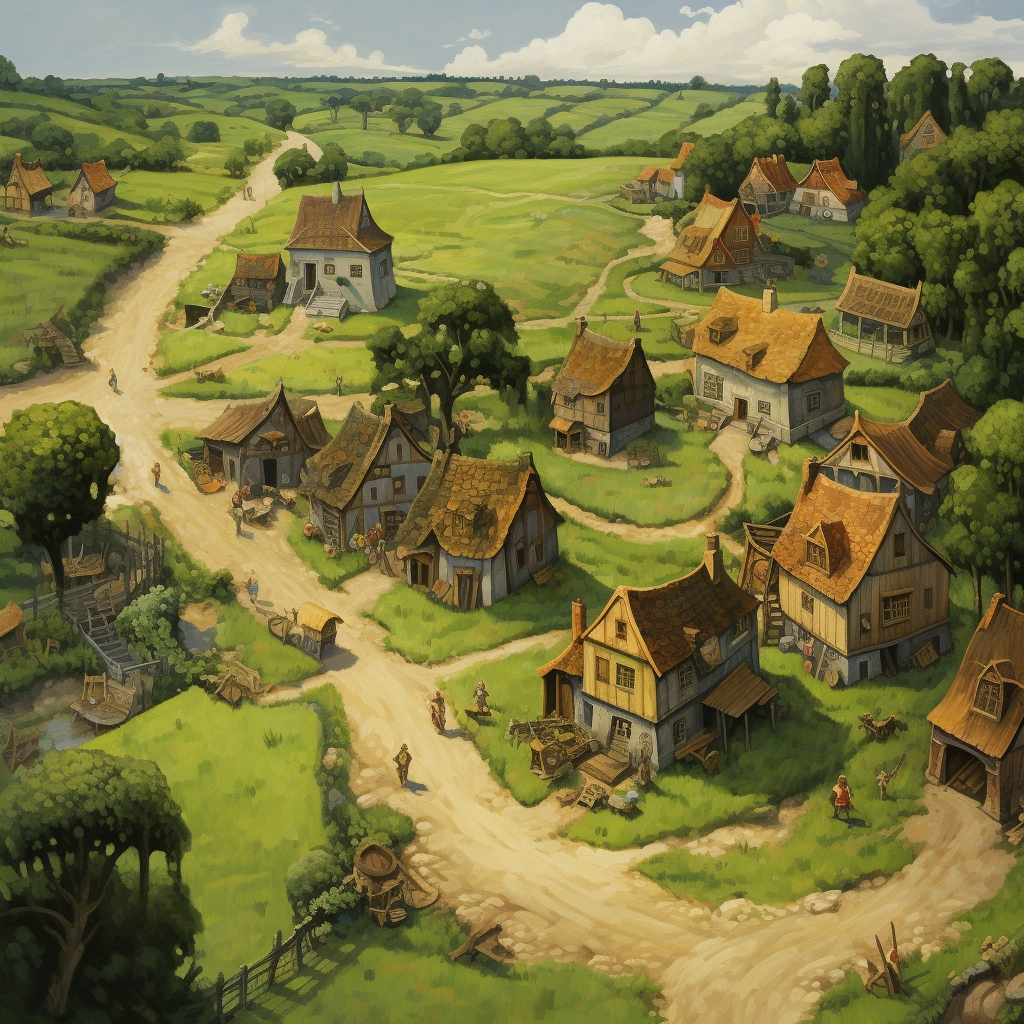
\includegraphics[scale=0.7]{BilderFuerBA/MeilensteinGebaude/a_scatch_from_a_village_top_down.png}
	\caption{a scatch from a village, top down}
	\label{fig:Midjourney-Conceptart-Dorf}
\end{figure}
Martin Luther, die Spielfigur in meinem Prototyp, soll sich am Ende durch ein Dorf bewegen und NPC treffen. In diesem Dorf befinden sich verschiedene Gebäude. In diesem Kapitel möchte ich zeigen, wie ich die Gebäude mit hilfe verschiedener KI-Systemen in der Unreal Engine 5 realisiert habe. Ich werde in diesem Kapitel und in den folgenden Meilensteine nicht mehr so detailliert alles wie bei der Erstellung der Hauptfigur, sondern nur auf Schritte eingehen, die im Prozess unterscheiden.
\\
Fachwerkhäuser repräsentieren etwas Mittelalterliches, und da die Renaissance an das Mittelalter zeitlich gegliedert ist, waren in Zeiten der Renaissance Fachwerkhäuser sehr weit verbreitet.
Meine Idee ist es, Diverse Fachwerkhäuser in meinem Dorf zu verteilen, um eine Dorflandschaft zu kreieren.
\\
Mein erster Ansatz ist, Häuser mit Hilfe von einem einfachen 3D-Modell umzusetzen, was ich in Blender erstellt habe. Dieses 3D-Modell bestand aus einem Quader mit einer Spitze. Kurz, ein einfaches Haus.
\\
Mit Midjourney habe ich Texturen erstellt, die Fachwerkhäuser nachempfunden sind. Diese Texturen und das einfache Haus wurden mit Hilfe von Blender verbunden. 
\\
Folgend wurden die einfachen Fachwerkhäuser in Unreal Engine 5 Importiert und verteilt.
\\
Die erste Version mit dem einfachen 3D-Modell ist ein Ansatz und hat funktioniert,  es für mein Prototyp nicht geeignet.  Dieser Ansatz wäre glaube ich gut geeignet, wenn.   Das Prototyp wenn der Spielcharaktere aus der isometrischen Sicht gesteuert wird, also von oben schräg und nicht aus der dritten Person, also von hinten über die Schulter klickend.  Wenn wir vor einem solchen Modell stets wirkt es doch sehr unglaubwürdig und unlebendig. Eine Inspiration für meinen zweiten Ansatz ist Walheim, ein Survivalspiel von den Coffee Stain Studios. In diesem Spiel gibt es ein Baukastensystem, in denen der Spieler sein eigenes Haus bauen kann.

Im Grunde genommen besteht ein Fachwerkhaus auch aus sebis simplen Bauteilen. Wie ZB wendebalken Dach. Ein Keller. Eine Treppe. Und diese einzelnen Elemente? 	Möchte ich nachbauen, so dass man im Unreal Engine Editor ein Haus selber bauen kann.  Der Vorteil dieser Methode liegt ganz klar auf der Hand. Zum Beispiel kann man mit Journey.  Immer wieder den gleichen Auftrag geben und er wird zum Beispiel von der Textur Stein. Immer wieder eine andere Textur ausgeben, die sich aber in sich ähneln, aber niemals gleichen.



Mein erster Ansatz war gut, aber nicht gut genug. Ich habe mich als ein Mann Videospiel Entwicklung gegen meinen ersten Ansatz entschieden. Nach der Implementierung in der Unreal Engine 5, sahen die 3D-Modelle für mein Geschmack etwas zu plastisch und platt aus. Die Balken innerhalb. Des Fachwerks haben keine Schatten geworfen und.  Sah einfach zu künstlich aus für meinen Geschmack. Also habe ich einen zweiten Ansatz entwickelt. Der zweite Ansatz besteht aus einem Baukastensystem, jeder Balken, jede Wand und jedes Dachelement hat.  Eine eigenes Element.  Diese Elemente können kann ich die diese Elemente, die in der Regel aus. Einfachen Formen wie?

Quader, oder?  	Dreiecke bestehen.  Kann ich einfach mit einem blueprint Skript.  Die Texturen jeweils. Hinzufügen.  Das bedeutet, ich brauche keinen Blender mehr, um ein 3 D Modell zu erzeugen, sondern mit einfachen.  Formen. Geometrien. Die über die andere Engine.   Mir zur Verfügung gestellt werden.  Mir einen einfachen Bausatz erstellen kann, die ich dann zusammengesteckt. Zusammenstecken kann. Um halt einfache Fachwerkhäuser. Zu erstellen.  Der Vorteil meines zweiten Ansatzes liegt darin, dass ich. Individuellere. Gebäude erstellen kann.

Die Sicherheit. Klar, auch in Form.  Von den Nachbarnhäusern unterscheiden.  	Ein weiterer Vorteil ist, ich kann Innenräumen gestalten, das in der ersten Version nicht. Möglich gewesen ist. Oder möglich ist.   	Ich kann mit der zweiten Version Innenräumen auch Fußboden gestalten. Ich kann Tapeten gestalten.


\subsection {Meilenstein: Nebenfiguren}
\subsection {Meilenstein: Dialogsystem}
\subsection {Meilenstein: Sprachausgabe}
\subsection{Erstellung von Musik und Klängen}
\subsection{Erstellung von Animationen}
\subsection{Entwicklung der Spiellogik}
%5
\section{Ergebnisse und Diskussion}
\subsection{Vorstellung des fertigen Videospiels}
\subsection{Diskussion der Ergebnisse und Einschätzung des Erfolgs des KI-Einsatzes}
\subsubsection{Einsatz von MonsterMash}
Monster Mash ist ein KI-System, mit dem man Monster erstellen kann. Wenn man sich realitätsnahe Ergebnisse wünscht, wird man mit Monster Mash auf sehr große Herausforderungen treffen.
\\
Monster sind Fantasiewesen, und niemand kann genau beschreiben, wie ein Monster aussieht. Bei der Darstellung von Menschen oder Gebäuden sieht das anders aus. Für mein Adventure-Game, mit einem historischen Hintergrund, ist MonsterMash nicht zu empfehlen.
\\
Anders würde es in einem Fantasy-Szenario aussehen, wo undefinierte Gestalten dem Spieler begegnen sollen.
\subsubsection{Einsatz von PFuHD}
PIFuHD ist eine KI-System was darauf trainiert ist, Digitalfotos von Personen in ein 3D-Modell umzuwandeln. PIFuHD kann man auf Google-Collab einrichten und lauffähig machen.
\\
Für das erstellen von 3D-Modellen wurde PIFuHD ist in der kostenlosen Demo-Version verwendet.
\\
Die Kompatibilität zwischen Midjourney und PIFuHD ist möglich. Die Resultate sind zum teil Artefakt belastet, die besonders in Bereichen der Hände, Füße und Kleidung auftreten.
\\
Durch Midjourney konnte ich Bilder von Martin Luther erzeugen, die als Konzeptgrafiken dienten. Diese Konzeptgrafiken habe ich PIFuHD als eingabe gegeben, und hat mir daraus folgende 3D-Modelle von Personen ausgegeben, die im Prototyp als Hauptfigur und NPCs verwendet wurden.
\subsection{Kritische Reflexion des Entwicklungsprozesses und Ausblick auf mögliche zukünftige Entwicklungen}
%6
\section{Fazit}
\subsection{Zusammenfassung der Ergebnisse}
\subsection{Implikationen für die Praxis}
\subsection{Limitationen der Studie}
%7
\section{Literaturverzeichnis}
%8
\section{Anhang}
\subsection{Abbildungen und Diagramme}
\subsection{Code-Beispiele}
\subsection{Weitere Materialien}
\end{document}





%\subsection{Nutzung von KIs zur Erstellung von 2D Bildern}
%Als erstes brauche ich eine Spielfigur die Martin Luther nachempfunden ist. Mein Worklfow besteht darin ein Promt von ChatGPT ausgeben zu lassen, den ich Später für Midjourney benutzen kann. Genau diesen Prompt habe ich ChatGPT übergeben.
